\documentclass{article}

\usepackage{authblk}
\usepackage{url}
\usepackage[square,numbers]{natbib}
\usepackage{color,amssymb,amsmath}
\usepackage{graphicx}
%\usepackage{graphicx}
%\SectionNumbersOn
%\AbstractOn

\title{A Natural Representation of Functions that Facilitates 'Exact Learning'}
%\author{Benedict W. J.~Irwin}


\date{\today}
\begin{document}
\bibliographystyle{harvard}

%\email{ben.irwin@optibrium.com}
%\affiliation{Optibrium, F5-6 Blenheim House, Cambridge Innovation Park, Denny End Road, Cambridge, CB25 9PB, United Kingdom}
%\alsoaffiliation{Theory of Condensed Matter, Cavendish Laboratories, University of Cambridge, Cambridge, United Kingdom}

\author[1,2]{Benedict W. J.~Irwin}
\affil[1]{Optibrium, F5-6 Blenheim House, Cambridge Innovation Park, Denny End Road, Cambridge, CB25 9PB, United Kingdom}
\affil[2]{Theory of Condensed Matter, Cavendish Laboratories, University of Cambridge, Cambridge, United Kingdom}
\affil[ ]{\textit {ben.irwin@optibrium.com}}


\maketitle

\begin{abstract}
We present a collection of mathematical tools and show a fundamental pattern across analytic functions that give a new perspective on machine learning with applications in all domains of science. This framework in principle allows the exact learning of functional forms and statistical distributions as solutions to natural problems arising in physics and mathematics by assuming they are drawn from a highly generalised class of functions. Such generalised representations have not yet been widely considered in the context of machine learning and data analysis. The full correlated probability distribution for inputs and outputs of a multivariate function can be learned under an analytic expansion in many variables. The moments of the distribution of choice are extracted using the generalised Ramanujan master theorem and training is directly applied to the coefficient function of the full probability distribution. The duality is manipulated through a multivariate Mellin transform which automatically handles the constraint of normalisation for probability distributions. These solutions use many fewer parameters than most machine learning methods and any method that connects these concepts successfully will likely carry across to non-exact problems and provide approximate solutions.

%We present a collection of mathematical tools that have great potential to enable innovations in machine learning. We communicate a fundamental pattern across analytic functions, which often arise as solutions to problems in all domains of science. A hierarchy of functions that follow this pattern reveals the kinds of trainable parameters that would be used for a machine learning model developed in this framework. A multivariate extension is considered for each of the functions in the hierarchy and how those representations might be more convenient and interpretable for the development of machine learning algorithms. 

%They could allow the exact learning of functional forms or statistical distributions which feature in natural problems arising in physics and mathematics using comparatively few parameters. The solutions drawn from highly generalized classes of functions have been documented rigorously in the space of special functions for mathematics, but have not yet have been considered by a wide audience for the purposes of machine learning and data analysis. There is reason that any method that could connect these concepts successfully would also carry across to non-exact problems and approximate solutions for use cases in traditional machine learning.

%The full correlated probability distribution for inputs and outputs of a multivariate function could be learned by assuming a highly generalised analytic expansion in many variables which is assumed to be described by a multivariate analogue of a highly generalised Meijer-G function, or analogous function which admits definition through a Barnes integral. 
%The moments of the distribution of choice are extracted using the generalised Ramanujan master theorem and training is directly applied to the coefficients of the full probability distribution. The duality is manipulated through a multivariate Mellin transform which can handle the constraint of normalisation for probability distributions.
\end{abstract}

%\tableofcontents

\section{Bigger Picture}
%A Bigger Picture statement should be 1 or 2 paragraphs with a maximum of 1,000 characters including spaces.

%Why is the research important?
%What are the longer-term ambitions of the research?
Can we use machine learning to help us solve equations and derive physical insight, without knowing anything about the origin of the data?
Often we can produce high precision numerical solutions to mathematical problems arising in many domains of science. These practically bypass solving intractable mathematical equations. How can we learn about the exact mathematical solution purely from the numerical output?

We first identify an important and natural way of encoding functions. This representations has been slowly developed over hundreds of years and great progress has been made in classifying functions in a general hierarchy. 

'Reverse Engineering', 'Experimental Mathematics'


This could be used to solve challenging integrals, differential equations and the form of distributions. Many integrals that relate to this method are studied in particle physics and string theory. 

%Does the research have the potential in the short or long term to make an impact on society?
This could facilitate automatic classification of curves. It may be applicable to machine learn unknown rules of nature given enough data.


\section{Introduction}
Machine learning (ML) is simplistically a form of 'function fitting' and ML methods often try to recreate a set of training observations by fitting a function to or 'learning from' example data points. The best method depends on the application and great success has been seen using this methodology on a range of problems across all domains of science and industry {\color{red}[CITE]}. One fundamental problem most ML methods is that the resulting functional form that fits to the data, is ultimately an approximation or interpolation of a restricted sample of points. Any learning that happens is then also in some sense restricted or limited to the domain of the training set or conditions in which the data were collected. The form chosen to fit the data is usually selected for convenience, convergence properties, speed or simplicity and the coefficients gained from the 'learning' process are likely to be somewhat arbitrary, not necessarily represent anything fundamental, and hard to interpret. In order to reach these high precision approximations, many parameters are required, sometimes millions or billions of parameters {\color{red}[CITE]}. This situation is likely 'non-physical' and unlikely to lead to transparent and understandable solutions which makes it hard for current ML methods to assist in the collection of natural facts. \\

True learning is timeless. If an exact solution to a problem exists, for example a solution to a particular differential equation, this solution is a permanent solution across the entire domain of applicability. This concept applies for problems from mathematics and physics where there is an unchanging 'ground truth' defined by nature. For example, {\color{red}[MORE EXAMPLES?], certain distributions of values in number theory problems}. \\


We will consider how 'machine learning like techniques' (i.e. advanced function fitting), can help with 'exact learning' type problems.
Specifically, the problem description is: "Given a high precision numeric output of an unknown function or distribution, write the 'human readable equation' for that function out". The concession we are willing to take is "Given a high precision numeric output of an unknown function or distribution, write the \emph{unique fingerprint} of the function". The key component here is the \emph{fingerprint} of an arbitrary function. This is essentially a reverse engineering process reminiscant of Simon Plouffe's "inverse symbolic calculator" in which a user would enter a high precision number e.g. "14.687633495788080676" and the algorithm would return a plausible closed form solution e.g. $\pi^2 + e\sqrt{\pi}$. Once we have the solution, the hope is that a human expert could come up with further insights which would assist in the scientific understanding.

Figure X demonstrates the flow.

[Image of functions going in to a box, and solutions coming out, introduce concept of an intermediary fingerprint]
\begin{figure}
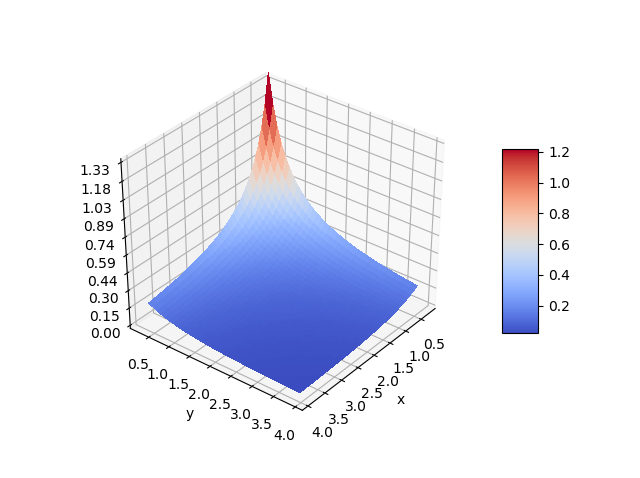
\includegraphics[scale = 1]{Distribution/2D.png}
\caption{}
\end{figure}


[Fractals are infinite compositions of analytic solutions]



An example might be a time independent wavefunction of a system from quantum mechanics. If a complicated potential is defined, it may be possible to numerically solve for the wavefunction to high precision in some parts of the domain. This gives a grid of numbers/data but does not translate to a permanent and unchanging piece of information, or fact of the universe. We try to establish a method that could suggest a mathematical form for such a numerical solution given enough data, without trying to solve an input system of equations, i.e. unsupervised exact learning.

To begin to phrase a machine learning problem in terms of exact functions, large changes need to be made to the underlying representation of the functions, and the network. In this work we introduce a mathematical scheme to attempt to do this based on the observation that many fundamental analytic functions are described within a special hierarchy.

The key message of this work is: "Let us turn our attention to the hierarchy of functions and associated methods, keeping machine learning in mind.". What algorithms can be developed from this? This intends to be a foundational paper that lays the concepts on the table but stops short of connecting them together. This is deliberate to avoid invoking the technical requirements that are needed for a solution. There are a number of potential engineering problems that may need to be overcome in terms of training networks that are constructed using these concepts.

Many of the references in this work are only hosted on pre-print servers such as the ArXiv and have not (yet) made it into journals. We applaud this ease of accessibility and take this to be a sign of the cutting edge.


Many of the tools developed here are treated in a highly rigorous or abstract mathematical way in the literature. While this is necessary for the correctness of the underlying mathematics, it reduces the accessibility of the concepts to those who have not invested as much time in developing the prerequisites and stymies innovation. In order to stimulate ideas surrounding these methods we have tried to reduce the complexity. We will introduce the necessary fundamentals with a higher level description. 


{\color{red} We suggest the name Ramanujan Master Process (RMP) for the prescription.

Nature has a non-arbitrary language. The coefficients of these functions have a clear role in the mathematical construction, and it is possible that closed form solutions, or tidy series solutions could in principle be found to fundamental problems expanding the domains of particle physics, statistical mechanics.

If we can find exact solutions to problems that allow it, there is a good chance any method that achieves this could also find approximate solutions to nosier problems.

Ramanujan Master Theorem. \citep{Gonzalez2015}
They show how the GMRT can be used to solve multivariate problems. This is the inverse of the machine learning, as the functions inside the integrals are known, but the solution to the integral is not. Nevertheless this connection is essential.

Many great ideas toward this are presented by Geenens \citep{Geenens2017} in much more mathematical detail. They develop flexible kernel density estimators using the moment properties of the Meijer-G function.

}

{\color{red} In this work we provide a high level overview of how one might construct a method to fulfil the goal of "". }

(Cite cosmology work.)


\section{Background and Method}
We will go through the background theory and arrangement of concepts to exactly learn the functional forms of high quality numeric data. As with other types of machine learning, fitting and optimisation problems, it is convenient to define a loss function $L$ that should be minimised to solve the problem. The gradient of the loss function will be taken with respect to parameters, and the training process will then resemble deep learning and will be compatible with existing software packages such as tensorflow and pytorch {\color{red} [CITE]}.
 
Our loss function will simply be the squared difference between the 'experimental fingerprint' of our numerical solution and the 'theoretical fingerprint' i.e the model we are trying to fit to the data. The question then becomes "what is the fingerprint of a function" and how do we measure this both experimentally and theoretically?

The fingerprint we use is the \textbf{Mellin transform} of a function or distribution. To understand the rational behind this we explain a pattern in a generalised representation of analytic functions.


\subsection{Nature's Language for Analytic Functions}
Many different types of mathematical function are used in quantitative branches of science. Because the language of mathematics is an \emph{ad hoc} set of notation which has evolved with time, it can be hard to keep a sense of order on named functions. Many people will be familiar with the functions $\exp(x)$ and $\log(x)$, which seem fundamental to nature and describe natural concepts such as exponential growth, order of magnitude and scale invariance. Many are familiar with trigonometric functions such as $\sin(x)$ for describing oscillation. In engineering and physics yet more complicated 'special functions' were developed for convenience, e.g. Bessel functions which can relate to cylindrical harmonics, along with various special (orthogonal) polynomials that describe spherical harmonics and so on.

The \emph{ad hoc} definition and naming of these functions cannot continue indefinitely, but analytic functions have power series expansions, many of which can be converted to a representation in terms of so-called \textbf{hypergeometric series}. A a core-component of this description is the Gamma function
\begin{equation}
\Gamma(s) = \int_0^\infty x^{s-1} e^{-x}dx,
\end{equation}
which is the continuous analogue to the factorial function $n!$. The Gamma function will be pivotal for our definition of a function's fingerprint.

Functions that could be described as a hypergeometric series could be represented as a limiting case of the 'hypergeometric function' which can be written in terms of ratios of gamma functions. We can write a definition of the hypergeometric function (with a negative argument) as
\begin{equation}
_2F_1(a,b;c;-x) = \sum_{s=0}^\infty \frac{(-1)^s}{s!} \frac{\Gamma(c)\Gamma(a+s)\Gamma(b+s)}{\Gamma(a)\Gamma(b)\Gamma(c+s)} x^s,
\label{eqn:hypergeom}
\end{equation}
where the striking component is the 'block' of $\Gamma$ functions. We will define the \emph{fingerprint} of the hypergeometric function as the so-called Mellin transform of the function 
\begin{equation}
\mathcal{M}\left[_2F_1(a,b;c;-x)\right](s) = \underbrace{\frac{\Gamma(c)\Gamma(a-s)\Gamma(b-s)\Gamma(s)}{\Gamma(a)\Gamma(b)\Gamma(c-s)}}_{Fingerprint}
\end{equation}
the fundamental pattern that we will exploit, is that for a huge variety of analytic functions, the fingerprint is described as a block of $\Gamma$ functions.

Some analytic functions \emph{cannot} be described by hypergeometric series. There are further extensions to the series definition which begin to describe these addition functions. This process of generalisation has iterated numerous times over the course of history, each time capturing successively more of the functions which are not described by the previous iterations. This is a neat and hierarchical way of describing this huge space of functions which we will use as a language for 'exact learning'.

The Mellin transform converts a function into its fingerprint and the \emph{inverse Mellin transform} transforms the fingerprint into the function. The inverse Mellin transform is a contour integral, that uses the residue theorem to recreate the series expansion of the function. The more generalised functions considered in this work are conveniently described in this way, which is called a Mellin-Barnes integral. For the hypergeometric function (equation \ref{eqn:hypergeom}) the corresponding definition through a Barnes integral is
\begin{equation}
_2F_1(a,b;c;-x) =\frac{\Gamma(c)}{\Gamma(a)\Gamma(b)} \frac{1}{2\pi i} \int_{-i\infty}^{i\infty} \frac{\Gamma(a+s)\Gamma(b+s)\Gamma(-s)}{\Gamma(c+s)}x^s\,ds
\end{equation}

{\color{blue}For a list of example functions that can be described by this method see Appendix XYZ. In short they range from a number of domains of science. The unifying feature of all of these series is their expression through a so-called Mellin-Barnes integral.}


{\color{red} For further discussion of the definition of these highly generalised functions ...}

{\color{red} \subsection{Highly Generalised Functions}
Here we will walk through some of the previously mentioned 'highly generalised functions', observe their similarities and differences and see how such differences change the kinds of functions that can be expressed. These functions assume an analytic series expansion and allow the coefficients of the series expansion to be altered through a minimal set of input parameters, usually denoted $a,b,c$ and so on. For certain sets of parameters, the series expansions for many common functions can arise. A list of early examples of these highly generalised functions can be found in well known texts [CITE]. Many of these functions have constraints on the combinations of arguments that can be used. For the sake of focus and scope in this text we will not mention any regions of convergence or the necessary analytic continuations in the following sections, but these should be considered carefully when such equations are implemented numerically. A careful treatment is given by ... et al. [CITE]. }







Geenens \citep{Geenens2017} derives a particular kernel density estimator using the Meijer-G function which can capture as limiting cases a number of common statistical distributions over a one dimensional domain, including Beta prime, Burr, Chi, Chi-squared, Dagum, Erlang, Fisher-Snedecor, Frechet, Gamma, Generalised Pareto, Inverse Gamma, Levy, Log-logistic, Maxwell, Nakagami, Rayleigh, Singh-Maddala, Stacy and Weibull. Geenens also gives an excellent summary of the mathematical properties of the Mellin transform and its applications to probability functions and some of the more technical details surrounding the Meijer-G function itself \citep{Geenens2017}.

\citep{Passare1996} Mellin-Barnes integrals and their applications in string theory, these authors give a very detailed analysis of the convergence criteria for Horn type series.



\section{Background}
The method begins with an observation that a large number of functions can be defined through a Mellin-Barnes integral over a product of gamma functions and their reciprocals. Functions defined in this manner have become increasingly generalised as time has passed to capture more and more special functions as limiting cases [CITE]. We review some necessary mathematical tools to describe the RMP method along with some generalised special functions and their Mellin transforms, which for suitably normalised distribution functions represent the moments of the distribution function:

\subsection{Mellin Transform}
Mellin transforms depend strongly on the so called 'strip of holomorphy' for a given function. This is covered in detail by Geenens \citep{Geenens2017}. A comprehensive table of Mellin transforms is given by [Caltech Integral Transforms] [CITE]. We define the Mellin transform as an integral transform of a function $f(x)$ as
\begin{equation}
\mathcal{M}[f(x)](s) = \int_0^\infty x^{s-1}f(x) dx = \varphi(s)
\end{equation}
which will obviously only converge for certain choices of functions $f(x)$ and certain exponents $s$. The set of complex values $s$ that converge for a function $f$ is the so called strip of holomorphy. It should be noted that if $f(x)$ is a probability distribution with positive semi-infinite support, through the definition of the Mellin transform we must have $\varphi(1)=1$ due to the normalisation constraint \citep{Geenens2017}. This concept will be used later to automatically train functions which can act as probability distributions. The inverse Mellin transform is given by
\begin{equation}
\mathcal{M}^{-1}[\varphi(s)](x) = \frac{1}{2 \pi i}\int_{c- i \infty}^{c + i \infty} x^{-s} \varphi(s) \; ds = f(x)
\label{eqn:InverseMT}
\end{equation}
where $i$ is the imaginary unit and the limits on the integral are to be interpreted as a line in the imaginary axis passing through a real constant $c$ which must lie in the strip of holomorphy and to the {\color{red}(left?)} of all poles in the function $\varphi(s)$. To avoid the complexity of such inverse transforms we use the Ramanujan master theorem (RMT) as a bridge to convert between a function $f(x)$ and its Mellin transform $\varphi(s)$.

\subsection{Ramanujan Master Theorem (RMT)}
The Mellin transform acts as a method of extracting the coefficients which define a particular series expansion of a function. The Ramanujan master theorem details how this extraction is achieved for suitably convergent functions and choices of exponent [CITE]. For suitable functions that admit a series expansion of the form
\begin{equation}
f(x) = \sum_{k=0}^\infty \chi_k \phi(k)x^k, \;\;\;\;\; \chi_k = \frac{(-1)^k}{k!}
\label{eqn:RMTSum}
\end{equation}
where $\chi_k$ is the alternating exponential symbol \footnote{If $\sum_i a_ix^i$ is a generating function and $\sum_i \frac{a_ix^i}{i!}$ is an \emph{exponential} generating function and if $\sum_{i} a_i$ is a sum and $\sum_i (-1)^i a_i$ is an \emph{alternating sum} it makes sense to call $\frac{(-1)^i}{i!}$ the alternating, exponential symbol.} the RMT states that the Mellin transform of the function is given by
\begin{equation}
\mathcal{M}[f(x)](s) = \Gamma(s)\phi(-s)
\end{equation}
where $\Gamma(s)$ is the Euler gamma function. This relationship sometimes relies on the analytic continuation of the coefficient function $\phi(s)$ to accept negative (and potentially complex) quantities. Functions whose $\phi(k)$ functions are ratios of Euler gamma functions are generally well behaved under continuation due to $\Gamma(s)$ being an almost entire function. This relationship holds very successfully for functions which admit definition through a so-called Barnes integral which is covered in section \ref{sec:BarnesIntegral}. In order to use the RMT as a bridge to avoid contour integrals of the type in equation \ref{eqn:InverseMT}, we should be able to work backwards. For a suitable \emph{unknown} function $f(x)$, if the Mellin transform $\varphi(s)$ is known, the function may admit reconstruction through equation \ref{eqn:RMTSum} which acts as an implicit inverse Mellin transform. Specifically
\begin{equation}
\mathcal{M}^{-1}[\varphi(s)](x) = \sum_{k=0}^\infty \frac{(-1)^k}{k!}\frac{\varphi(-k)}{\Gamma(-k)}x^k = f(x)
\label{eqn:ImplicitInverseMellin}
\end{equation}
where often the $\Gamma(-k)$ term will directly cancel if the Mellin transform $\varphi(s)$ contains a simple factor of $\Gamma(s)$. At this point it might be helpful to see some tangible examples of this in action. We direct the reader to {\color{red} Appendix 1} for such examples.


\subsection{Table of Functions Using $\Xi$ Notation}
For the hierarchy of special functions considered in this work, it is convenient to define a "product gamma" operation $\Xi[\cdot]$ which flattens a vector or matrix and takes a product of the gamma function over the elements. The use of this custom operation will make the pattern between the functions easier to see. Table \ref{tab:Xi} shows how the operation works for vector and matrix arguments and with an optional exponent vector to realise products of powers of gamma functions. This can be easily extended for any array of higher dimensions. Define for a vector $\mathbf{v}$ or matrix $\mathbf{V}$ of exponents of equal size.
\begin{table}
\begin{tabular}{|c|c|c|}
\hline
Input & Vectors $\mathbf{a,v} \in \mathbb{R}^D$ & Matrices $\mathbf{A,V} \in \mathbb{R}^D\times \mathbb{R}^D$ \\
\hline
No Exponent & $\Xi[\mathbf{a}] = \prod_{k=1}^D \Gamma(a_k)$ & $\Xi[\mathbf{A}] = \prod_{k=1}^D\prod_{l=1}^D \Gamma(A_{kl})$ \\
Exponent & $\Xi^\mathbf{v}[\mathbf{a}] = \prod_{k=1}^D \Gamma^{v_k}(a_k)$ & $\Xi^\mathbf{V}[\mathbf{A}] = \prod_{k=1}^D\prod_{l=1}^D \Gamma^{V_{kl}}(A_{kl})$\\
\hline
\end{tabular}
\caption{Table explaining the $\Xi$ operation on different inputs with and without vector exponents.}
\label{tab:Xi}
\end{table}

\section{Mellin Transforms of Hierarchy of Functions}
All of the functions in this natural description can be defined as a Mellin-Barnes integral [CITE] in the form
\begin{equation}
f(x) = \frac{1}{2\pi i}\int_L z^s \bar{\phi}(s)\;ds
\end{equation}
for a suitable definition of $\bar{\phi}$ [CITE]. $L$ is a special contour path which is covered in detail in references defining each function [CITE]. The fundamental pattern is that for many classes of functions $\bar{\phi}$ is expressed as a product of gamma functions and their reciprocals. This is a method of encoding the series expansion in terms of the residue theorem, where the contour $L$ encircles poles which contribute to the series expansion of $f(x)$. The function $\bar{\phi(s)}$ is related to the Mellin transform of $f(x)$ by inverting the sign of $-s$. 

The hierarchy of these highly generalised series is presented in Table 2 with the function definition and the associated Mellin transform (i.e. the moments). The progression in terms of complexity advances down the table, through the hypergeometric function and its generalisation [CITE], the Fox-Wright series and its normalised counterpart [CITE], the highly flexible Meijer-G function [CITE] and its analogous extension the Fox-H function [CITE]. We include two more recent, extremely general extensions, the Inayat-Hussain-$\bar{H}$ [CITE] and the Rathie-I function [CITE]. We note that Rathie has also extended to even more generalised functions \citep{Rathie2013} which are discussed in section ({\color{red} XYZ Deep learning}), and this table is not necessarily exhaustive. Functions such as the MacRobert-E function bridge the gap between hypergeometric and Meijer-G  type functions in the table. 

{\color{red} Mention the heirarchy of functions}

The hierarchy in table 2 progresses in terms of complexity by first adding shift parameters to the arguments of the gamma functions. Then the number of gamma functions is increased, and vector shift parameters $\mathbf{a,b,c,d}$ are used. We switch to the $\Xi$ notation from table 1 at this point to retain compact expressions. Next the inclusion of vector scale parameters, $\mathbf{e,f,g,h}$, extend from hypergeometric functions to Meijer-G functions, which gives a large boost to the types of function that can be represented (see Appendix {\color{red}XYZ}). The most general functions come from adding vector power parameters $\mathbf{i,j,k,l}$, which begin to describe extremely complex physical and number theoretic functions [CITE], (see Appendix {\color{red}XYZ, to ... and ...}).


The Meijer-G function suffers from an unfortunate notation where the vectors of parameters are split. It is convenient to rewrite the two vectors of parameters, as four individual vectors of parameters for a consistent hierarchy. We note that the sign of the argument is reversed in the Meijer-G function definition. Here we include a scale factor $\eta$ on the variable for extra generalisation. 


%Mellin transform of the H-function: https://arxiv.org/pdf/1302.2954.pdf
\begin{table}
\begin{tabular}{|c|c|c|c|}
\hline
Function Name & $f(x)$ & $\varphi(s)=\mathcal{M}[f(x)](s)$ & Reference \\
\hline
Hypergeometric & $_2 F_1 \!\left( \left. \begin{matrix} a,b \\ c \end{matrix} \; \right| \, -\eta x \right)$ & $\eta^{-s}\frac{\Gamma(c)\Gamma(a-s)\Gamma(b-s)}{\Gamma(a)\Gamma(b)\Gamma(c-s)}\Gamma(s)$ & \\
Generalised Hypergeometric &  $_p F_q \!\left( \left. \begin{matrix} \mathbf{a} \\ \mathbf{b} \end{matrix} \; \right| \, -\eta x \right)$ & $\eta^{-s}\frac{\Xi[\mathbf{b}]\Xi[\mathbf{a}-s\mathbf{1}]}{\Xi[\mathbf{a}]\Xi[\mathbf{b}-s\mathbf{1}]}\Gamma(s)$ &  \\
Fox-Wright-$\Psi$ & $_p\Psi_q \!\left[\left.\begin{matrix}
\mathbf{a},\mathbf{e} \\
\mathbf{b},\mathbf{f} \end{matrix} \;\right| -\eta x  \right]$ & $\eta^{-s}\frac{\Xi[\mathbf{a}-s\mathbf{e}]}{\Xi[\mathbf{b}-s\mathbf{f}]}\Gamma(s)$ & \\
Fox-Wright-$\Psi^*$ & $_p\Psi_q \!\left[\left.\begin{matrix}
\mathbf{a},\mathbf{e} \\
\mathbf{b},\mathbf{f} \end{matrix} \;\right| -\eta x  \right]$ & $\eta^{-s}\frac{\Xi[\mathbf{b}]\Xi[\mathbf{a}-s\mathbf{e}]}{\Xi[\mathbf{a}]\Xi[\mathbf{b}-s\mathbf{f}]}\Gamma(s)$ & \\
\hline
Meijer-G & $G_{p,q}^{\,m,n} \!\left( \left. \begin{matrix} \mathbf{a,b} \\ \mathbf{c,d} \end{matrix} \; \right| \, \eta x \right)$ & $\eta^{-s}\frac{ \Xi[\mathbf{1}-\mathbf{a}-s\mathbf{1}]\Xi[\mathbf{c}+s\mathbf{1}]} {\Xi[\mathbf{1}-\mathbf{d}-s\mathbf{1}]\Xi[\mathbf{b}+s\mathbf{1}]}$& \\
Fox-H & $H_{p,q}^{\,m,n} \!\left[\left. \begin{matrix}
\mathbf{a},\mathbf{b},\mathbf{e,f} \\
\mathbf{c},\mathbf{d},\mathbf{g,h} \end{matrix} \right| \eta x \right]$ & $\eta^{-s}\frac{\Xi[\mathbf{1-a}-s\mathbf{e}]\Xi[\mathbf{c}+s\mathbf{g}]}{\Xi[\mathbf{1-d}-s\mathbf{h}] \Xi[\mathbf{b} + s \mathbf{f}]}$ & \citep{Fox1961,Rathie2017}\\
Inayat-Hussain-$\bar{H}$  & $\bar{H}_{p,q}^{\,m,n} \!\left[\left. \begin{matrix}
\mathbf{a},\mathbf{b},\mathbf{e,f,i} \\
\mathbf{c},\mathbf{d},\mathbf{g,h,l} \end{matrix} \right| \eta x \right]$ & $\eta^{-s}\frac{\Xi^{\mathbf{i}}[\mathbf{1-a}-s\mathbf{e}]\Xi[\mathbf{c}+s\mathbf{g}]}{\Xi^{\mathbf{l}}[\mathbf{1-d}-s\mathbf{h}] \Xi[\mathbf{b} + s \mathbf{f}]}$ & \citep{InayatHussain}\\
Rathie-I & $I_{p,q}^{\,m,n} \!\left[\left. \begin{matrix}
\mathbf{a},\mathbf{b},\mathbf{e,f,i,j} \\
\mathbf{c},\mathbf{d},\mathbf{g,h,k,l} \end{matrix} \right| \eta x \right]$ & $\eta^{-s}\frac{\Xi^{\mathbf{i}}[\mathbf{1-a}-s\mathbf{e}]\Xi^{k}[\mathbf{c}+s\mathbf{g}]}{\Xi^{\mathbf{l}}[\mathbf{1-d}-s\mathbf{h}] \Xi^{\mathbf{j}}[\mathbf{b} + s \mathbf{f}]}$ & \citep{Rathie1997}\\
\hline
\end{tabular}
\caption{A table of generalised special functions and their Mellin transforms. Small bold letters are vectors of parameters where $\mathbf{a,b,c,d}$ are shift factors, $\mathbf{e,f,g,h}$ are scale factors and $\mathbf{i,j,k,l}$ are exponents for the gamma functions, $\mathbf{1}$ represents a vector of all 1's. Complexity increases down the table which is split into an upper part for hypergeometric functions and a lower part for Meijer-G like functions.}
\end{table}


\subsection{Conclusions from Generalised functions}
\begin{enumerate}
\item We have seen that the most generalised functions in mathematics already employ the Mellin duality for their definition.
\item These functions have grown interest in the evaulation of Feynman integrals from QED and QFT.
\item The core component is products of Euler gamma functions and their reciprocals.
\item Scale parameters on the moments inside the gamma functions are justified.
\item Powers of gamma functions are justified in some of the more advanced definitions.
\item Scale terms for the arguments of functions are expressed as very simple terms in the moment function.
\end{enumerate}


\section{Multiple Dimensions}
Most machine learning problems require learning a function of more than one variable. The previous section dealt with increasingly generalised definition of functions in one dimensional domain. A similar set of tools can be developed for functions with a $D$ dimensional domain.

\subsubsection{Multivariate Moment Functional}
Firstly, for convenience of notation define the a \emph{multivariate moment functional} which can be seen as a vectorised power operation that acts on two length $D$ vectors as
\begin{equation}
\mathbf{a}^\mathbf{b}_\Pi = \prod_{l=1}^D {a_l}^{b_l}
\end{equation}
which returns a scalar value. This operation will conveniently vectorise the ensuing equations. It is clear to see by the fundamental rules of exponentiation that $\mathbf{a}^\mathbf{b}_\Pi\mathbf{a}^\mathbf{c}_\Pi = \mathbf{a}^{\mathbf{b+c}}_\Pi$.  In this notation the multivariate moment of a vector of quantities $x$ and a vector of exponents $s$ is simply $\mathbf{x}^\mathbf{s}_\Pi$

\subsection{Multivariate Mellin Transform}
In analogy to the multivariate Fourier and Laplace transforms one can define a multivariate Mellin transform [CITE]. For $\mathbf{x} \in \mathbb{R}^D$ we define the multivariate Mellin transform as the integral transform
\begin{equation}
\mathcal{M}_D[f(\mathbf{x})](\mathbf{s}) = \int_{[0,\infty)^D} \mathbf{x}^\mathbf{s-1}_\Pi f(\mathbf{x}) d \mathbf{x} = \varphi(\mathbf{s})
\end{equation}
where $d\mathbf{x} = dx_1 \cdots dx_D$. The inverse transform is a multiple complex contour integral representation [CITE] but an exact form will not be needed due to the generalised Ramanujan master theorem (GRMT).

\subsection{Generalised RMT (GRMT)}
The GRMT takes the analogous problem of solving the \textit{multivariate} Mellin transform of a function with a vector input which is expressed through an analytic series expansion. The GRMT and associated 'method of brackets' has been covered in a series of work from {\color{red}Gonzales et al.} \citep{Gonzalez2015} which covers the definition and historical developments [CITE], application of the GRMT to special functions from G\&R [CITE] and solving laborious and complicated integrals from quantum field theory \citep{Gonzalez2011}. If a function $f(\mathbf{x})$ admits a series expansion (using a vector multi-index $\mathbf{k}$),  \begin{equation}
f(\mathbf{x}) = \sum_{\mathbf{k}=0}^\infty \chi(\mathbf{k}) \phi(\mathbf{k}) \mathbf{x}^{\mathbf{A}\mathbf{k}+ \mathbf{b}}_\Pi
\end{equation}
with multivariate coefficient function $\phi(\mathbf{k})$, a $D\times D$ matrix of exponent weights $\mathbf{A}$ and a vector of exponents $\mathbf{b} \in \mathbb{R}^D$, and with multivariate alternating exponential symbol
\begin{equation}
\chi(\mathbf{k}) = \left(\prod_{l=0}^D \chi_{k_l}\right),\;\;\;\;\; \chi_k = \frac{(-1)^k}{\Gamma(k+1)}
\end{equation}
then the multivariate Mellin transform of $f(\mathbf{x})$ is given by the expression \begin{equation}
\mathcal{M}_D[f(\mathbf{x})](\mathbf{k}^*) = \frac{\phi(\mathbf{k}^*)}{|\det(\mathbf{A})|} \prod_{l=1}^D \Gamma(-k_l^*) = \frac{\phi(\mathbf{k}^*)\Xi[-\mathbf{k}^*]}{|\det(\mathbf{A})|}
\end{equation}
where $\mathbf{k}^*$ is the solution to $\mathbf{A}\mathbf{k^*}+\mathbf{s}=\mathbf{0}$ \citep{Gonzalez2015}. This is a very powerful equation which can be used to solve many high dimensional integrals from quantum electrodynamics \citep{Gonzalez2011}.

\section{Multidimensional Hypergeometric Series}
Here we define a hypergeometric series analogue which extends into multiple dimensions. Many such functions have been investigated for two dimensions including the Horn, Appell ... [CITE], for three dimensions including Lauricella [CITE] and further [CITE]. For the purposes of this work we will generalise in the following way:

\begin{enumerate}
\item Write the one dimensional series of choice in terms of gamma functions using the alternating exponential character.
\item Replace the variable term $x^k$ with $\mathbf{x}^{\mathbf{A}\mathbf{k}}_\Pi$ for a variables fully coupled with all indices.
\item Replace the alternating exponential character $\chi_k$ with the multivariate character $\Pi\chi(\mathbf{k})$.
\item Replace the products of ratios of gamma functions with the following:
\begin{enumerate}
\item $\Gamma(a) \to \Xi[\mathbf{a}]$.
\item $\Gamma(s) \to \Xi[\mathbf{s}^*]$.
\item $\Gamma(a+s) \to \Xi[\mathbf{a}+\mathbf{A}\mathbf{s}]$.
\end{enumerate}
\end{enumerate}

Define the product of gamma functions over a vector of arguments operator
\begin{equation}
\Xi[\mathbf{x}] = \prod_{l=1}^D \Gamma(x_l)
\end{equation}


\section{Extracting the Moments from a Generalised Probability Distribution}
Here we show how the application of the GRMT to a general analytic probability distribution. This motivates the choice of a product of gamma functions and shows that the arguments of those functions contain the solutions to a matrix equation which relates to the [{\color{red} Jacobian of the variables}, proof].

\subsubsection{Generalised Distribution}
Suppose we have a distribution $P(\mathbf{x})$ where both input variables and output variables are treated equally as terms in $\mathbf{x}$. Suppose these inputs and outputs are all in the positive real numbers. The fundamental assumption behind the RMP is to assume a multivariate analytic expansion of this distribution in terms of a set of coefficients $\varphi$. Assume a form for the multivariate distribution, using a vector index notation $\mathbf{k} = (k_1, \cdots, k_n)$ where the sum extends from $0$ to $\infty$ for each index
\begin{equation}
P(\mathbf{x}) = \sum_{\mathbf{k}=0}^\infty  \Pi\chi(\mathbf{k})\varphi(\mathbf{k})\mathbf{x}^{\mathbf{A}\mathbf{k}+\mathbf{b}}_\Pi
\end{equation}
where the $\mathbf{a}_l$ are row vectors of a matrix $\mathbf{A}$ whose coefficients describe the relationship between the variables $\mathbf{x}$ and the summation indices $\mathbf{k}$, the $b_l \in \mathbf{b}$ are constant terms in the exponents of the variables, $f(\mathbf{k})$ is a multivariate coefficient function which defines the moments of the probability distribution. We may write the expectation of a given multivariate moment as a function of the vector of exponents of the variables $\mathbf{s}$
$$
\mathcal{E}_P(\mathbf{s}) = \mathbb{E}\left[\prod_{k=0}^n X_k^{s_k-1}\right] = \mathbb{E}\left[\Upsilon(\mathbf{X},\mathbf{s}-\mathbf{1})\right] =\int_{[0,\infty)^{n}} \Upsilon(\mathbf{x},\mathbf{s}-\mathbf{1}) P(\mathbf{x}) \; d \mathbf{x}
$$
where the $\mathbf{s}-\mathbf{1}$ has been included to make the expression match the definition of a multivariate Mellin transform. As a consequence by the GRMT this is representable in terms of the divergent bracket symbols of [Gonzalez et. al] \citep{Gonzalez2015}, which they define as
\begin{equation}
\langle s \rangle = \int_0^\infty x^{s-1} \; dx
\end{equation}
which are used to \emph{formally} manipulate the series expansion according to their rules. Note that due to separability the integral of a product of variables to exponents is simply a product of bracket symbols
\begin{equation}
\int_{[0,\infty)^n} \mathbf{x}^{\mathbf{s-1}}_\Pi\;d \mathbf{x} = \prod_{l=1}^n \int_0^\infty x_l^{s_l-1} \; dx_l = \prod_{l=1}^n \langle s_l \rangle
\label{eqn:bracket}
\end{equation} 


We may write explicitly using vector arguments for brevity
\begin{equation}
\mathcal{M}_P(\mathbf{s}) = \int_{[0,\infty)^{n}} \mathbf{x}^{\mathbf{s-1}} \sum_{\mathbf{k}=0}^\infty  \chi(\mathbf{k})\varphi(\mathbf{k}) \mathbf{x}^{\mathbf{A}\mathbf{k}+\mathbf{b}}_\Pi \; d \mathbf{x}
\end{equation}
under linearity bring the product of variables under the summation sign and combine it with the variables being summed over
\begin{equation}
\mathcal{M}_P(\mathbf{s}) = \int_{[0,\infty)^{n}} \sum_{\mathbf{k}=0}^\infty  \chi(\mathbf{k})\varphi(\mathbf{k}) \mathbf{x}^{\mathbf{s-1}}_\Pi \mathbf{x}^{\mathbf{A}\mathbf{k}+\mathbf{b}}_\Pi \; d \mathbf{x}
\end{equation}
\begin{equation}
\mathcal{M}_P(\mathbf{s}) = \int_{[0,\infty)^{n}} \sum_{\mathbf{k}=0}^\infty  \chi(\mathbf{k})\varphi(\mathbf{k})\mathbf{x}^{\mathbf{A}\mathbf{k}+\mathbf{b}+\mathbf{s-1}}_\Pi \; d \mathbf{x}
\end{equation}
swapping the sum and the integral under linearity would give
\begin{equation}
\mathcal{M}_P(\mathbf{s}) = \sum_{\mathbf{k}=0}^\infty  \chi(\mathbf{k})\varphi(\mathbf{k})\int_{[0,\infty)^{n}} \mathbf{x}^{\mathbf{A}\mathbf{k}+\mathbf{b}+\mathbf{s-1}}_\Pi \; d \mathbf{x}
\end{equation}
using equation \ref{eqn:bracket} we can convert these to divergent bracket symbols
\begin{equation}
\mathcal{M}_P(\mathbf{s}) = \sum_{\mathbf{k}=0}^\infty  \chi(\mathbf{k})\varphi(\mathbf{k}) \prod_{l=1}^n \langle \mathbf{a}_l \cdot \mathbf{k} + \mathbf{b} + \mathbf{s} \rangle
\end{equation}
according to rule 2[{\color{red} verify the number}] of Gonzalez et al. [CITE] this summation can be written by the GRMT as 
\begin{equation}
\mathcal{M}_P(\mathbf{s}) = \frac{\varphi(\mathbf{k}^*) \prod_{l=0}^n \Gamma(-k_l^*)}{|\det(\mathbf{A})|}
\end{equation}

for $k^*_m$ as the values that satisfy the linear system of equations by vanishing the set of $\langle \cdot \rangle$ brackets. That is the solution to \begin{equation}
\mathbf{A}\mathbf{k}^*+\mathbf{b}+\mathbf{s} = \mathbf{0}
\end{equation} 

This means under a suitable definition of $\varphi$ we have an expression for all of the moments of the probability distribution.
\subsection{A Form for $\varphi$}
By observations in the literature and the discussion in sections \ref{} and \ref{} that show families of highly generalised functions can be characterised by moments which are expressed purely as rations of gamma functions and their reciprocals, we are motivated to select a form for $\varphi$ that is comprised of gamma functions. As shown in section \ref{}, scale factor terms on variables are separable under the Mellin transform. We can observe the following classes of choices of $\varphi$ \begin{enumerate}
\item $\varphi$ with a product of ratios of gamma functions whose arguments are simple shift equations of linear sums of unscaled indices. These are likely to describe probability distributions drawn from the family of generalised hypergeometric functions and Meijer-G functions.
\item $\varphi$ with a product of ratios of gamma functions whose arguments are simple shift equations of linear sums of \emph{scaled} indices. These are likely to be drawn from a family of functions resembling the Fox-H function.
\item $\varphi$ with a product of ratios of gamma functions \emph{raised to real powers} whose arguments are simple shift equations of linear sums of \emph{scaled} indices. This are likely to express probability distributions that are selected from the [{\color{red} I-function and H-bar function}] family of functions.
\end{enumerate}


\subsection{What Problems Could be Solved}
The types of problem that can be solved must produce high quality numerical data. Obvious candidates are numerical integration or the numerical solution to differential equations. Others might be Monte-Carlo simulations that produce a distribution or function.




Complex Problem: Generates Distribution or curve. How to fit a function to this without solving the equations.

Quantum mechanics.


\section{Comparison to a Neural Network}
Equation X shows that the moments of a multivariate distribution were connected to the 'block' of gamma functions through the MDMT and GRMT. The logarithm of these moments is given by
\begin{equation}
\log \mathcal{M}[P(\mathbf{x})](\mathbf{k}) = \beta - \log(\varphi(\mathbf{k}^*)) - \sum_{l=0}^n \log\Gamma(-k_l^*)
\end{equation}
where $\beta = \log(|\det(\mathbf{A})|)$ is a constant for a given $\mathbf{A}$ and if $\phi(\mathbf{k})$ is of the highly generalised form of the Rathie-I function
\begin{equation}
\phi(\mathbf{k}) =  \eta^{-s}\frac{\Xi^{\mathbf{i}}[\mathbf{1-a}-s\mathbf{e}]\Xi^{k}[\mathbf{c}+s\mathbf{g}]}{\Xi^{\mathbf{l}}[\mathbf{1-d}-s\mathbf{h}] \Xi^{\mathbf{j}}[\mathbf{b} + s \mathbf{f}]}
\end{equation}
we can compare this to the equations for a neural network with input vector $\mathbf{x}$, one activation layer and aa single output $y$.
\begin{equation}
y = \mathbf{w}\cdot\sigma(\mathbf{Ax} + \mathbf{b}) + c
\end{equation}
we see a mapping between $c \to \beta$, $\sigma(\cdot) \to \log\Gamma(\cdot)$, $\mathbf{Ax + b} \to \mathbf{k}^*$, and $\mathbf{x} \to \mathbf{k}$. The final weight layer $\mathbf{w}$, represents the power of the gamma functions (and therefore whether that term is on the top or bottom of the block). We then conclude that one possible interpretation of a neural network is an attempt to approximate the output variable as the log-moments of a multivariate distribution.

Moreover, if the bias in the final layer is close to zero, the correlation of descriptors is ...

[Display a plot of ReLU, Tanh and LogGamma]

It may be sensible to add regularisation terms to this loss, for example ({\color{red}$\Delta$, the discriminant from string theory paper}), and the normalisation constraint for probability distributions.

\section{Comparison to a Deep Neural Network}
It is possible to (trivially) write the gamma function itself as a contour integral \citep{Rathie2013}. 

\begin{equation}
\Gamma(z) = \frac{1}{2\pi i}\int_L \frac{\Gamma(s)\Gamma(z)}{\Gamma(1+s)} ds
\end{equation}

If the Mellin transform, of a function or distribution is analogous to the moments, then a second iteration of that process is the moments of the moments. 

\section{An Example}
Consider a mathematical problem that generates an unknown distribution that we wish to know more about. We uniformly generate a random point in a unit circle centred at the origin. We also uniformly generate a random point in the unit square bounding $x,y \in [0,1]$. Take the distance between the points and consider the probability $P(d)$ of finding a pair of points separated by a distance $d$. Of course there are methods to solve this using pen and paper, but we will instead apply the {\color{red}Ramanujan Master Process} and find a solution.

First we collect high precision data. We generate 10 million pairs, calculate the distance, and plot a histogram (Figure Xa), next we calculate the expectation $E[x^{s-1}]$, for $100$ values of $s$ sampled uniformlyin $s \in [1,4]$ (Figure Xb). We can take the log moments which are simply $\log(E[x^{s-1}])$ (Figure Xc). Then we fit a function using the log-Gamma ($\mathrm{l}\Gamma = \log\Gamma$) function of the form
\begin{equation}
\log(E[x^{s-1}]) = s \log(\alpha) + \log(\beta) + \mathrm{l}\Gamma(s) + \left(\sum_{k=1}^{K_+}\mathrm{l}\Gamma(s + a_k)-\mathrm{l}\Gamma(a_k)\right)  - \left(\sum_{k=1}^{K_-}\mathrm{l}\Gamma(s + b_k)-\mathrm{l}\Gamma(b_k)\right)
\end{equation}
where $K_+$ is the number of positive terms, and $K_-$ is the number of negative terms, these correspond to gamma functions on the top and bottom of the block respectively. The best fit was found for $(K_+=...)$, (Figure Xd). The sum of square differences for the fit is $5.24 \times 10^{-9}$.

We vary the number of terms and attempt the fit each time, in effect we are fitting a hypergeometric type function to the distribution.

We can then conclude that 
\begin{equation}
\int_0^\infty x^{s-1}p(x) \; dx  \approx \alpha^s \cdot \beta \Gamma(s)\frac{\Gamma(a)\Gamma(c)\Gamma(b+s)}{\Gamma(b)\Gamma(a+s)\Gamma(c+s)}
\end{equation}
implying
\begin{equation}
p(x) = \beta _2F_1(1-a,1-b,1-c;\frac{x}{\alpha})
\end{equation}

Consider the orderings.

\subsection{Robbins Constant}
We see a similar behaviour with the problem.

\subsection{Other Strategies}
Sometimes we have a sum of the functions?
Inverting the function? Residue summation?

\subsection{Variation of Solution}
We can consider the problem and vary inputs to the problem and look at the changes in the solution. The gradients will help us numerically identify cases where parameters have certain relations. For example if 

\begin{equation}
\frac{\partial}{\partial \alpha} \log M[f](s,\alpha) \approx A\frac{s}{\alpha}
\end{equation}
then we can identify that $\alpha$ is a simple scale factor on the final solution. If we have \begin{equation}
\frac{\partial}{\partial \alpha} \log M[f](s,\alpha) \approx \psi^{(0)}(a+s) - \psi^{(0)}(s)
\end{equation}
then there is a term 
\begin{equation}
\frac{\Gamma(a+s)}{\Gamma(a)}
\end{equation}
in the moments.

\subsection{Some Numeric Tests}
\subsubsection{1D- Exponential}
We generated $1000$ samples from the distribution $x_1 \sim \exp(-x)$. The algorithm was run for $1000$ epochs which went beyond convergence. The final parameters were $V = [0.00132615]$ and $a=[1.0014696]$. In 1-D we may approximate this as \begin{equation}
\tilde{F}^{(1)}(1;;0,;x) = \sum_{k=0}^\infty \frac{(-1)^k}{k!} \frac{\Gamma(1+0k)}{\Gamma(1)} x^k = e^{-x}
\end{equation}
the original distribution is recreated for this extremely simple case.


\section{Conclusions}
We presented the following concepts: 1) A Barnes integral defining a function over a 'block' of gamma functions; 2) The Mellin transform connecting the analytic expansion of such a function to that 'block' of gamma functions; 3) A natural hierarchy of 1-D special functions that can be defined in this way progressing through hypergeometric, generalised hypergeometric, Fox-Wright, Meijer-G, Fox-H, Inayat-Hussain-H and Rathie-I functions which correspond to increasingly complex changes to the arguments and powers of gamma functions in the 'block', but also an increasingly expanding set of representable natural functions which appear as solutions to problems across many domains of science.


In order to connect these components methods will be required to train over large products of gamma functions and their ratios, for which logarithmic expressions may help. If the log-gamma function is seen as an activation function, the expression for the log moments of functions defined by the procedure represent the layers of a neural network. If gradients are to be used the mathematical expressions are tractable and contain digamma functions. Problems may arise for negative arguments due to the presence of the poles.

There are functions whose moments cannot be expressed by a 'block' of gamma functions, but instead by generalised functions themselves. We believe further more generalised fitting procedures can be developed to incorporate these solutions into the method.




\section{Acknowledgements}
B.W.J.I. acknowledges a portion of the research was made during his time in the EPSRC Centre for Doctoral Training in Computational Methods for Materials Science for funding under grant number EP/L015552/1. B.W.J.I is grateful for Optibrium Ltd. for giving him the freedom to further develop these concepts alongside his role there.







\section{Appendix 1: Examples of the Mellin Transform and RMT}
\subsubsection{Negative Exponential}
One of the simplest functions to use as an example is $f(x)=e^{-x}$, the Mellin transform of this is
\begin{equation}
\mathcal{M}[e^{-x}](s) = \int_0^\infty x^{s-1}e^{-x} \; dx = \Gamma(s)
\end{equation}
which can be seen to be an integral definition of the Euler gamma function. If we look at the series expansion of $e^{-x}$ we have
\begin{equation}
e^{-x} = \sum_{k=0}^\infty \frac{(-1)^k}{k!} x^k = \sum_{k=0}^\infty \chi_k \phi(k) x^k
\end{equation}
here we see that the coefficient function $\phi(k)$ is always $1$. Which by the RMT predicts the Mellin transform of $e^{-x}$ to be
\begin{equation}
\mathcal{M}[e^{-x}](s) = \Gamma(s)\phi(-s) = \Gamma(s)\cdot 1 = \Gamma(s)
\end{equation}
which is in agreement with the integral definition.
\subsubsection{Binomial $(1+x)^{-1}$}
We can consider the function $f(x) = \frac{1}{1+x}$ with expansion
\begin{equation}
\frac{1}{1+x} = \sum_{k=0}^\infty \frac{(-1)^k}{k!} k! x^k = \sum_{k=0}^\infty \chi_k \Gamma(k+1) x^k
\end{equation}
here the continuation of the coefficient function $\phi(k) = \Gamma(k+1)$. We can use the RMT to predict that the Mellin transform is
\begin{equation}
\mathcal{M}\left[\frac{1}{1+x}\right](s) = \Gamma(s)\phi(-s) = \Gamma(s)\Gamma(1-s)
\end{equation}
if we evaluate the integral directly this is the case.
\subsubsection{Binomial $(1+x)^{-a}$}
As before we write the series expansion
\begin{equation}
\frac{1}{(1+x)^a} = \sum_{k=0}^\infty \binom{-a}{k} x^k = \sum_{k=0}^\infty \chi_k \frac{\Gamma(k+a)}{\Gamma(a)} x^k
\end{equation}
Then the Mellin transform by the RMT is 
\begin{equation}
\mathcal{M}\left[\frac{1}{(1+x)^a}\right](s) = \frac{\Gamma(s)\Gamma(a-s)}{\Gamma(a)}
\end{equation}

\section{Appendix 2: Miscellaneous}
\subsection{Multivariate Functions}
To train on datasets with more than one column we will require multivariate analogues of the special functions. Huge collections of multivariate definitions have been collected by Horn, Lauricella, Appell, Kampe-de-Feriet etc.[CITE]. Undoubtedly many more have been considered in recent times. For the purposes of defining a clear rule for this work we directly transform the expressions in table \ref{} using a collection of simple rules using the $\Xi$ and multi-power notation.

\subsubsection{Appell $F_1$ Function}
This can be written as a double contour integral
\begin{equation}
F_1(a;b_1,b_2;c;z_1,z_2) = \frac{1}{(2\pi i)^2}\int_{L^*} \int_L  \bar{\phi}(s,t) (-z_1)^{-s_1}(-z_2)^{-s_2} ds_1 ds_2
\end{equation}
with \begin{equation}
\bar{\phi}(s_1,s_2) = \frac{\Gamma(c)\Gamma(a-s_1-s_2)\Gamma(b_1-s_1)\Gamma(b_2-s_2)\Gamma(s_1)\Gamma(s_2)}{\Gamma(a)\Gamma(b_1)\Gamma(b_2)\Gamma(c-s_1-s_2)}
\end{equation}
Which some parts can be rewritten as 
\begin{equation}
\bar{\phi}(s_1,s_2) = \frac{\Xi[c])\Xi[a-\mathbf{1}\cdot\mathbf{s}]\Xi[\mathbf{b}-\mathbf{s}]\Xi[\mathbf{s}]}{\Xi[a]\Xi[\mathbf{b}]\Xi[c-\mathbf{1}\cdot\mathbf{s}]}
\end{equation}
the function is defined with $\mathbf{M}=\mathbf{I}_2$ which has determinant $1$. Because of this we know that $\mathbf{k}^* = -\mathbf{s}$, this explains the $\Xi[\mathbf{s}]$ term.

If this is to bee seen as a conversions from a 1-D function to a 2D function we will start from a hypergeometric function. To cover the general case, a few matrices might be needed:
\begin{table}
\begin{tabular}{|c|c|}
\hline
Before & After \\
\hline
$a$ & $a$ \\
$b$ & $\mathbf{b}=(b_1,b_2)$ \\
$c$ & $c$ \\
$s$ & $\mathbf{s} = (s_1,s_2)$ \\
\hline
$\Gamma(a)$ & $\Gamma(a)$\\
$\Gamma(b)$ & $\Xi[\mathrm{b}]$ \\
$\Gamma(c)$ & $\Gamma(c)$\\
\hline
$\Gamma(a-s)$ & $\Gamma(a - \mathbf{1}\cdot\mathbf{s})$\\
$\Gamma(b-s)$ & $\Xi[\mathbf{b-s}]$ \\
$\Gamma(x-s)$ & $\Gamma(c - \mathbf{1}\cdot\mathbf{s})$\\
\hline
\end{tabular}
\caption{Table showing transforms from a 1-D hypergeometric function with $3$ parameters to a 2-D Appell hypergeometric with $4$ parameters. }
\label{tab:1dto2d}
\end{table}

From table \ref{tab:1dto2d} we can see that there is a delicate balance between parameter vectors with changing numbers of parameters and the change in dimensionality.

\subsubsection{Gauss Hypergeometric to Lauricella Function in N-D}
There are four Lauricella functions in $D$ dimensions [CITE]. The function of type-A for example is
\begin{equation}
F_A^{(n)}(a, b_1,\ldots,b_n, c_1,\ldots,c_n; x_1,\ldots,x_n) = 
\sum_{i_1,\ldots,i_n=0}^{\infty} \frac{(a)_{i_1+\ldots+i_n} (b_1)_{i_1} \cdots (b_n)_{i_n}} {(c_1)_{i_1} \cdots (c_n)_{i_n} \,i_1! \cdots \,i_n!} \,x_1^{i_1} \cdots x_n^{i_n}
\end{equation}
One can conceive a higher generalisation of this which should be one of the most general (at the expense of additional parameters). Define
\begin{equation}
\tilde{F}^{D}(\mathbf{a};\mathbf{b};\mathbf{V,W};-\boldsymbol\eta \odot\mathbf{x}) = \sum_{\mathbf{k}} \chi(\mathbf{k})\frac{\prod_{j=1}^D (a_j)_{\mathbf{v}_j \cdot \mathbf{k}}}{\prod_{j=1}^D (b_j)_{\mathbf{w}_j \cdot \mathbf{k}}} \boldsymbol\eta^{\mathbf{k}}_\Pi\mathbf{x}^{\mathbf{k}}_\Pi
\end{equation}
which in terms of gamma functions is 
\begin{equation}
\tilde{F}^{D}(\mathbf{a};\mathbf{b};\mathbf{V,W};-\boldsymbol\eta \cdot\mathbf{x}) = \sum_{\mathbf{k}} \chi(\mathbf{k})\frac{\prod_{j=1}^D \Gamma(b_j)\Gamma(a_j + \mathbf{v}_j\cdot \mathbf{k})}{\prod_{j=1}^D \Gamma(a_j)\Gamma(b_j+\mathbf{w}_j\cdot \mathbf{k})} \Upsilon(\boldsymbol\eta,\mathbf{k})\Upsilon(\mathbf{x},\mathbf{k})
\end{equation}
which in terms of $\Xi$ is
\begin{equation}
\tilde{F}^{D}(\mathbf{a};\mathbf{b};\mathbf{V,W};-\boldsymbol\eta \cdot\mathbf{x}) = \sum_{\mathbf{k}} \chi(\mathbf{k})\frac{\Xi[\mathbf{b}]\Xi[\mathbf{a}+\mathbf{Vk}]}{\Xi[\mathbf{a}]\Xi[\mathbf{b+Wk}]} \Upsilon(\boldsymbol\eta,\mathbf{k})\Upsilon(\mathbf{x},\mathbf{k})
\end{equation}
because $\mathbf{M}=\mathbf{I}_D$ by the GRMT the Mellin transform is equal to \begin{equation}
\mathcal{M}[\tilde{F}^{D}(\mathbf{a};\mathbf{b};\mathbf{V,W};-\boldsymbol\eta \cdot\mathbf{x})](s) = \frac{\Xi[\mathbf{b}]\Xi[\mathbf{a}-\mathbf{Vs}]}{\Xi[\mathbf{a}]\Xi[\mathbf{b-Ws}]}\Xi[\mathbf{s}]\Upsilon(\boldsymbol\eta,-\mathbf{s})
\end{equation}
in this way there is no need for a determinant which is an obstruction to training. From this standpoint the original series is reclaimable. One question is whether is is necessary to add an additional matrix $\mathbf{M}$ at all.

\section{Multidimensional Generalised Hypergeometric Function}
For the 1D generalised hypergeometric function we have $\mathbf{a} \in \mathbb{R}^p$, $\mathbf{b} \in \mathbb{R}^q$ and $\mathbf{x} \in \mathbb{R}^n$. In the $\Xi$ and multi-power notation
\begin{equation}
_pF_q(\mathbf{a};\mathbf{b};-\mathbf{x}) = \sum_{\mathbf{k}}\chi(\mathbf{k})     \left(\prod_{l=1}^n \frac{\prod_{m=1}^q \Gamma(b_{lm})}{\prod_{m=1}^p \Gamma(a_{lm})} \frac{\prod_{m=1}^p \Gamma(a_{lm} + \alpha_l \cdot \mathbf{k})}{\prod_{m=1}^q \Gamma(b_{lm} + \alpha_l \cdot \mathbf{k})} x_l^{\alpha_l \cdot \mathbf{k}}\right)
\end{equation}
here we notice the $\mathbf{a}$ and $\mathbf{b}$ are essentially matrices. The corresponding choice of $f$ is
\begin{equation}
f(\mathbf{k},\cdots) = \prod_{l=1}^n \frac{\prod_{m=1}^q \Gamma(b_{lm})}{\prod_{m=1}^p \Gamma(a_{lm})} \frac{\prod_{m=1}^p \Gamma(a_{lm} + \alpha_l \cdot \mathbf{k})}{\prod_{m=1}^q \Gamma(b_{lm} + \alpha_l \cdot \mathbf{k})}
\end{equation}
this form is potentially more useful. We now have two parameters we can control, $p$ and $q$. These parameters control the complexity of the fitted function given a number of dimensions. It is usually the case that $p=q+1$ for the one dimensional hypergeometric functions. This then gives the generalised Mellin transform:
$$
...
$$

\section{Multi-Dimensional Meijer-G Function}
Likewise we may consider defining a multi-dimensional variant of the Meijer-G function. Consider the Mellin transform of a Meijer-G function with a scale parameter $\eta$:

\begin{equation}
\int_0^{\infty} x^{s - 1} \; G_{p,q}^{\,m,n} \!\left( \left. \begin{matrix} \mathbf{a_p} \\ \mathbf{b_q} \end{matrix} \; \right| \, \eta x \right) dx =
\frac{\eta^{-s} \prod_{j = 1}^{m} \Gamma (b_j + s) \prod_{j = 1}^{n} \Gamma (1 - a_j - s)} {\prod_{j = m + 1}^{q} \Gamma (1 - b_j - s) \prod_{j = n + 1}^{p} \Gamma (a_j + s)}
\end{equation}
this means
\begin{equation}
G_{p,q}^{\,m,n} \!\left( \left. \begin{matrix} \mathbf{a_p} \\ \mathbf{b_q} \end{matrix} \; \right| \, \eta x \right) = \sum_{s=0}^\infty \frac{(-1)^s}{s!} \frac{1}{\Gamma(s)} \frac{\prod_{j = 1}^{m} \Gamma (b_j - s) \prod_{j = 1}^{n} \Gamma (1 - a_j + s)} {\prod_{j = m + 1}^{q} \Gamma (1 - b_j + s) \prod_{j = n + 1}^{p} \Gamma (a_j - s)} (\eta x)^s
\end{equation}

\subsubsection{Replacement Rules}

\begin{enumerate}
\item For scalar constants, $\Gamma(a) \to \Xi[\mathbf{a}]$, where $a$ becomes a vector $\mathbf{a}$ which is indexed over dimensions.
\item For vectors indexed over parameters, $\Xi[\mathbf{a}] \to \Xi[\mathbf{A}]$, where $\mathbf{a}$ becomes a matrix $\mathbf{A}$ which is indexed over parameters and dimensions.
\item For scale constants, $\eta^{-s} \to \mathbf{\boldsymbol\eta}^{-\mathbf{s}}_\Pi$.
\item For variables in integrands $x^k \to \mathbf{x}^{\mathbf{Ak}}_\Pi$
\item In series the alternating exponential character becomes the multivariate alternating exponential character: $\chi_k \to \Pi\chi(\mathbf{k})$
\end{enumerate}

\begin{table}
\begin{tabular}{|c|c|c|}
\hline
Before & After & Notes \\
\hline
$\Gamma(a)$ & $\Xi[\mathbf{a}]$ & $a \in \mathbb{R} \to \mathbf{a} \in \mathbb{R}^D$\\
$\Gamma(a \pm k)$ & $\Xi[\mathbf{a}\pm \mathbf{k}]$ & $a,k \in \mathbb{R} \to \mathbf{a},\mathbf{k} \in \mathbb{R}^D$\\
$\Xi[\mathbf{a}]$ & $\Xi[\mathbf{A}]$ & \\
$\Xi[\mathbf{a}\pm s \mathbf{1}]$ & $\Xi[\mathbf{A} ??]$ & \\
\hline
$x^k$ & $\Upsilon[\mathbf{x},\mathbf{Mk}]$ & \\
$(\eta x)^k$ & $\Upsilon[\boldsymbol\eta,\mathbf{Mk}]\Upsilon[\mathbf{x},\mathbf{Mk}]$ & \\
\hline
$\chi_k$ & $\Pi\chi(\mathbf{k})$ & \\
$k$ & $\mathbf{k}$ & \\
$\sum_{k=0}^\infty$ & $\sum_{k_1=0}^\infty \cdots \sum_{k_D=0}^\infty$ & \\
\hline
\end{tabular}
\caption{Table for transformation rules from a function in one variables to a function in multiple variables.}
\end{table}

\subsubsection{Note:}
We do not apply the transformation rule $\Gamma(a+k) \to \Xi[\mathbf{a} + \mathbf{Mk}]$ because upon solving the GMRT we find the Mellin transform contains terms such as $\Xi[\mathbf{a} + \mathbf{Mk^*}]$ which is equal to $\Xi[\mathbf{a} - \mathbf{s}]$ by the definition of $\mathbf{k}^*$. The resulting Mellin transform is separable in terms of the elements of $\mathbf{s}$ which shows the resulting distribution is a product of marginal distributions i.e. uncorrelated random variables, which is not ideal for machine learning. If $\mathbf{M}=\mathbf{I}_D$ then the distribution is separable which could be learned for distributions with that property.

\subsubsection{Example: Multivariate Hypergeometric Function}
Here we perform the above prescription to convert the hypergeometric function to the multivariate hypergeometric function. We have the one dimensional hypergeometric function.
\begin{equation}
_2F_1(a,b;c;-\eta x) = \sum_{k=0}^\infty \chi_k \frac{\Gamma(c)\Gamma(a+k)\Gamma(b+k)}{\Gamma(a)\Gamma(b)\Gamma(c+k)} (\eta x)^k
\end{equation}
For the higher dimensional versions we write the equivalent definition
\begin{equation}
_2\mathbf{F}_1(\mathbf{a},\mathbf{b};\mathbf{c};-\boldsymbol\eta\odot\mathbf{x}) = \sum_{\mathbf{k}}\Pi\chi(\mathbf{k})\frac{\Xi[\mathbf{c}]\Xi[\mathbf{a}+\mathbf{k}]\Xi[\mathbf{b}+\mathbf{k}]}{\Xi[\mathbf{a}]\Xi[\mathbf{b}]\Xi[\mathbf{c}+\mathbf{k}]}{(\boldsymbol\eta\odot\mathbf{x})}^{\mathbf{M}\mathbf{k}}_\Pi
\end{equation}
with the Hadamard product $\odot$. From the GRMT we know the generalised Mellin transform of this multidimensional analogue to the hypergeometric function is equal to
\begin{equation}
\int_{[0,\infty)^n}\mathrm{x}^{\mathbf{s-1}}_\Pi\;_2\mathbf{F}_1(\mathbf{a},\mathbf{b};\mathbf{c};-\mathbf{x})\; d\mathbf{x} = \frac{\phi(\mathbf{k}^*)\Xi[-\mathbf{k}^*]}{|\det(\mathbf{M})|}
\end{equation}
which based on equation \ref{} is \begin{equation}
\mathcal{M}_D[_2\mathbf{F}_1(\mathbf{a},\mathbf{b};\mathbf{c};-\mathbf{x})] = \frac{\Xi[\mathbf{c}]\Xi[\mathbf{a}+\mathbf{k}^*]\Xi[\mathbf{b}+\mathbf{k}^*]\Xi[-\mathbf{k}^*]}{\Xi[\mathbf{a}]\Xi[\mathbf{b}]\Xi[\mathbf{c}+\mathbf{k}^*]|\det(\mathbf{M})|}
\end{equation}
where $k^* = -\mathbf{M}^{-1}\mathbf{s}$.

%noting that if 
%\begin{equation}
%\mathbf{A}\mathbf{k^*}+\mathbf{s} = \mathbf{0}
%\end{equation}
%it is clear to see that $\mathbf{A}\mathbf{k^*} = \mathbf{-s}$ giving
%\begin{equation}
%\mathcal{M}_D[_2\mathbf{F}_1(\mathbf{a},\mathbf{b};\mathbf{c};-\mathbf{x})] = \frac{\Xi[\mathbf{c}]\Xi[\mathbf{a}-\mathbf{s}]\Xi[\mathbf{b}-%\mathbf{s}]\Xi[-\mathbf{k}^*]}{\Xi[\mathbf{a}]\Xi[\mathbf{b}]\Xi[\mathbf{c}-\mathbf{s}]|\det(\mathbf{A})|}
%\end{equation}
%{\color{red} but this means the moments are separable? Which means the distribution is a product of marginals? Actually setting the rule $\Gamma(a+k) \to \Xi[\mathbf{a}+\mathbf{k}]$ doesn't lead to separated distributions. This might be the right way forward. The parameters in the gammas are aligned to the summation indices. The exponents of the variables are transformed by the matrix!}

\subsection{Appendix: List of Representable Functions}
Generalization of the Mittag-Leffler function \citep{Rathie2017}, expressible as $_1F_q$ and $H^{1,1}_{1,2}$.
$$
\frac{e^x}{3} + \frac{2 e^{-x/2}}{3}\cos(\frac{\sqrt{3}x}{2})
$$ \citep{Rathie2017}, expressible as $_0F_2$,$H^{1,1}_{1,2}$


The inverses for high order polynomials are ...
\citep{Irwin2017}

More advanced functions, i.e. number theory.
and ""Polylogarithms of complex order"" \citep{Rathie1997}

Feynman Integrals led to many developments. [InayatHussain1987]. Allowing machine learning to access this language could even help with problems in particle physics.

Statistical Mechanics: \citep{Rathie1997}, functions which cannot be represented as an H-function. 

""""E.g. in the case of the free energy of
a Gaussian model of phase transition,see Joycee (1972), in statistical mechanics
as given by Inayat-Hussain (1987)""" \citep{Rathie1997} \citep{Inayat Hussain 1987}

and """The Mellin-Barnes integral representation in the case of the Feynman
integral g, for non-integer m, as expressed in the following form, see InayatHussain (1987):"""


Method of moments!
Further generalised to continuous moments. 
Assumes the Hypergeometric representation.... 


"""Inayat-Hussain
(1987)."""

"""Also Hm n
p q is the H -function, see Fox (1961), Braaksma (1964), Mathai and
Saxena (1978)."""

"""Also Gm n
p q is the G-function, see Luke (1969)"""


Hypergeometric relations and Meijer-G functions have become popular in behind the scenes manipulations in computer algebra systems such as Mathematica [CITE]. Numerous algorithms are developed to try to look up the results to evaluate integrals [Peasgood]. \citep{Rathie1997}

"""Gamma, Psi and generalized Zeta functions. These methods have been
applied to various problems involving the derivation of the exact distribution
of the likelihood ratio criterion, see Anderson (1984). Among the first papers
in this direction, see Mathai and Rathie (1970, 1971)""" \citep{Rathie1997}


"""The well known H -function of one variable, defined by Fox (1961) and
studied by Braaksma (1964)""" \citep{Rathie1997}

\begin{table}
\begin{tabular}{|c|c|c|}
\hline
Hypergeometric Representation & Common Expression & Name\\
\hline
$_0F_0(;;z)$&$e^z$ &\\
$_1F_0(a;;z)$ & $(1-z)^{-a}$ &\\
$\frac{(\frac{x}{2})^\alpha}{\Gamma(\alpha+1)} _0F_1(;\alpha+1;\frac{-x^2}{4}) $ & $J_\alpha(x)$ & Bessel J \\
$\frac{(\frac{x}{2})^\alpha}{\Gamma(\alpha+1)} _0F_1(;\alpha+1;\frac{x^2}{4}) $ & $I_\alpha(x)$ & Bessel I \\
$_1F_1(a,;b;z)$ & $M(a;b;z)$ & Confluent Hypergeometric functions \\
$_1F_1(a;b;z)$ & $L$ & Laguerre polynomials \\
$_1F_1(a;b;z)$ & $H$ & Hermite polynomials\\
$_2F_1$ & & Legendre Polynomials\\
$_2F_1$ & & Spherical Harmonics \\
$_2F_0()$ & $Ei(z)$ & Exponential Integral \\
$_3F_0$ & $M$ & Mott polynomials \\
$x_3F_2(1,1,1;2,2;x)$ & $\mathrm{Li}_2(x)$ & Dilogarithm \\
3F2 & & Clebsch-Gordan coefficients \\
\hline
\end{tabular}
\caption{Some examples of hyper-geometric representations of common functions.}
\end{table}

Functions expressible by the Meijer-G function include sin,cos,sinh,cosh, arcsin, arctan, arccot, log(1+x), Heaviside step functions, the upper and lower incomplete gamma functions $\Gamma(\alpha,x)$ and $\gamma(\alpha,x)$, and their $\alpha$-derivatives. All Bessel functions of the first and second kind and thier modified forms, $J_\nu(x)$,$Y_\nu(x)$,$I_\nu(x)$,$K_\nu(x)$. Lerch transcendent $\Phi(x,n,a)$, {\color{red} and therefore the Hurwitz zeta function, Polylogarithm $\mathrm{Li}_s(z)$, Riemann zeta function, Dirichlet eta function and Legendre chi function}.

\begin{table}
\begin{tabular}{|c|c|c|}
\hline
Function & Mellin Transform\\
\hline
$e^{-x^n}$ & $n^{-1}\Gamma(\frac{s}{n})$ \\
$\log(1+x)$ & $s^{-1}\Gamma(s)\Gamma(1-s)$ \\
$J_n(x)$ & $2^{s-1}\frac{\Gamma(\frac{n}{2}+\frac{s}{2})}{\Gamma(1+\frac{n}{2}-\frac{s}{2})}$ \\
$Y_n(x)$ & $ $ \\
$K_n(x)$ & $2^{s-2}\Gamma(\frac{s}{2}-\frac{n}{2})\Gamma(\frac{s}{2}+\frac{n}{2})$ \\
\hline
\end{tabular}
\caption{Example of Mellin transforms of common functions yielding gamma functions.}
\end{table}



\subsection{Citations To Include}
\begin{enumerate}
\item Generalised Beta distributions show ratios of gamma functions. Make it possible to represent (elliptic?) or generalisations of the Dirchlet eta function? Alog with generalisations of the zeta function \citep{ostrovsky2013theory}.
\item This seems to show ratios of extended gamma functions etc. can have powerful expressions \citep{Luo2013}.
\item Rathie: %A.K. Rathie, A new generalization of generalized hypergeometric functions, Le Matematiche
%52 (1997), no. 2, 297 – 310.
\end{enumerate}
The convenient relationship with the Mellin transform is that scale parameters for the primary inputs can easily be added.


\citep{Rathie2013}
Rathie 2013 : Extremely generalised functions.
https://arxiv.org/pdf/1302.2954.pdf


Rathie 2017 summarises:

References pFq
[1] Bailey WN. Products of generalized hypergeometric series. Proc. London Math. Soc.
1928;28(2):242–254.
[2] Srivastava HM, Qureshi MI, Quraishi KA and Singh R. Applications of some hypergeometric
summation theorems involving double series. J Appl Math Statist Inform. 2012;8(2):37–48.
[3] Choi J, Rathie AK. On a Hypergeometric Summation Theorem due to Qureshi et al. Commun.
Korean Math. Soc. 2013; 28(3):527-534.
[4] Srivastava HM, Qureshi MI, Quraishi KA and Arora A. Applications of summation theorems
of Kummer and Dixon involving double series. Acta Mathematica Scientia. 2014;34(3):619–
628.


Mathai AM, Saxena RK and Haubold HJ. The H-function: Theory and Applications. New
York (NY): Springer; 2010.
[6] Springer MD. The Algebra of Random Variables. New York (NY): John Wiley; 1979.



The so-called Ramanujan Master Process (RMP) we present here relies on an assumed analytic multivariate series expansion of a function or distribution, which can be defined by its coefficients. 

In this method the representation of the coefficients is trained, however, coefficients are not trained individually but the whole set of coefficients are trained simultaneously. This will be achieved by exploiting a duality facilitated by the Mellin transform. Analogous to the way the Fourier transform links a periodic signal in time with a signal in the frequency domain, or a probability density function (p.d.f) with its characteristic function, the Mellin transform can be thought of as a transform from a p.d.f to its generalised moment function (distinct from the moment generating function). \par

\begin{equation}
\begin{matrix}
\hline
\mathrm{Waveform}(\mathrm{time}) & \underbrace{\longrightarrow}_{\mathrm{Fourier Transform}} & \mathrm{Spectrum}(\mathrm{frequency})\\
\hline
\mathrm{Distribution}(\mathrm{variable}) & \underbrace{\longrightarrow}_{\mathrm{Mellin Transform}} & \mathrm{Moments}(\mathrm{exponents}) \\
\hline
\end{matrix}
\end{equation}

Figure 1 is a schematic showing the analogy between these concepts. Just as the frequency is a continuous variable, the moment is a continuous variable. 


[Include a mention of the Laplace method summing up series, and the reproducing kernel Hilbert space.]


{\color{red}
\section{Important Equations}
\begin{equation}
\mathcal{M}\left[\Theta[1-x]\left(\sum_{k=0}^\infty c_k x^k \right)\right](s) = \sum_{k=0}^\infty \frac{c_k}{s+k}
\end{equation}
\begin{equation}
\mathcal{M}\left[\Theta[n-x]\left(\sum_{k=0}^\infty c_k  x^k \right)\right](s) = \sum_{k=0}^\infty \frac{c_k n^{s+k}}{s+k}
\end{equation}
\begin{equation}
\mathcal{M}\left[\Theta[1-x]\left(\sum_{k=0}^\infty c_k \log^k(x) \right)\right](s) = \sum_{k=0}^\infty \frac{(-1)^k k! c_k}{s^{k+1}}
\end{equation}



\section{Solution of Differential Equation}
In principle this could be used to find exact solutions in terms of moments of differential equations. Consider the Schrödinger equation.

\section{Solution of Numerical Integration}
With the modern power of numerical integration methods, it can be quite efficient to evaluate a whole bunch of integrals. Take for example the integral
\begin{equation}
I(a,b,c) = \int_0^1 \frac{dx}{\sqrt[3]{a x + b x^2 + cx^3}}
\end{equation}
which would be tricky to evaluate analytically. We can measure this to high precision numerically for a range of  values of $a,b,c$. And from this we measure the variation of the solution with respect to each parameter.

\section{Other Mathematical Processes}
Consider a complicated statistical or physical process. For example a simple molecular forcefield applied to a compound which undergoes non-simple dynamics.


\section{Comments}
Arguments may need to become complex numbers! This is important for optimisations. 
}


\section{References}
\bibliography{bibliography}


\end{document}